\chapter{Correspondencia con un problema de búsqueda.}\label{cap:capitulo6}

Hasta ahora hemos visto los elementos y el procedimiento del sistema para generar una solución válida. En este capítulo, analizaremos los elementos de un problema de búsqueda y los identificaremos en el sistema propuesto. Destacar que este trabajo, se ha necesitado un componente de aleatoriedad, por lo que el sistema construido no es totalmente fiel al método de búsqueda como tal, pero sí se basa de forma coherente en el mismo.

\section{Método de búsqueda}

Cuando se nos propone un problema en el que podemos conocer el \emph{espacio de soluciones}, se puede aplicar un método de búsqueda para la obtención de una de ellas que se ajuste al enunciado del problema. Así, el problema de búsqueda se puede constatar como encontrar una solución o estado concreto entre un conjunto de soluciones (el llamado \emph{espacio de estados}) que satisfaga el enunciado del problema.

Para transitar entre estados, y realizar la búsqueda de una solución adecuada, definiremos las \emph{acciones sobre estados}. De esta forma, realizaremos dichas acciones sobre los estados para obtener nuevos estados definidos en el \emph{espacio de estados}, y así poder indagar sobre el mismo para encontrar una solución factible para nuestro enunciado.

Así, analizaremos el problema de búsqueda desde el punto de vista de \emph{agentes} que realizan dicha búsqueda para encontrar una solución factible. En nuestro caso, podemos identificar el \emph{agente} como el sistema de generación que se ha elaborado.

\section{Modelización del problema}

El método de búsqueda se aplica a la resolución de problemas para los que existe un \emph{espacio de estados}. Para resolver el problema, se emplea un modelo del mismo, generalmente para simplificar y eliminar complejidad innecesaria. A partir de este modelo, se elaborará una estructura de datos que será la base para la resolución del modelo. Según la adecuación del modelo al problema real, así se adecuará la solución que encontremos, ya que la misma será una solución al modelo del problema, y no al problema en sí. Una elección de un modelo inadecuado, puede resultar en soluciones ineficientes.

En nuestro caso, se comentó la estructura de datos para la modelización del problema en el capítulo X (ENLACE A CAPITULO DE REPR. DEL MAPA). A partir de esta representación, se elaboró un sistema que iteraba sobre ella para ir construyendo una solución (ENLACE A CAPITULO DE ESTRATEGIA CONSTRUCTIVA), y es en la interfaz de construcción donde reside el resto de la similitud del sistema con una búsqueda.

\section{Búsqueda informada}

En este tipo de métodos, podemos encontrar una clasificación que divide entre \emph{búsqueda informada} y \emph{búsqueda no informada}. La \emph{búsqueda no informada} parte de que no se conoce información acerca del entorno en el que se realiza la búsqueda.

Por contrapartida, la \emph{búsqueda informada} se constata cuando sí podemos conocer en alguna medida el entorno en el que buscamos nuestra solución. La adecuación de la solución al enunciado del problema, dependerá del objetivo que se inste en el enunciado. Así, la búsqueda procurará encontrar una solución tomando este objetivo como baza para la obtención de la misma. Estos objetivos son los que denominaremos \emph{bondad}, \emph{fitness} o \emph{heurística} de la solución, y son los que nos guiarán en la búsqueda para la obtención de una solución adecuada al enunciado.

En este capítulo trataremos el método de \emph{búsqueda informada}, debido a que en nuestro problema, partimos de una serie de objetivos bien definidos y computables sobre los estados que componen el espacio de estados.

\section{Problemas resolubles mediante búsqueda}

Para que un problema sea abarcable por un método de búsqueda necesitamos que cumplan varias propiedades. Dichas propiedades, definiran de forma concisa un entorno en el que podamos utilizar el método, que requieren que el problema esté bien definido según las mismas.

El problema debe ser \emph{discreto}, es decir, el espacio de estados debe estar \emph{bien definido} y ser \emph{finito}. Además, esto conlleva que el número de \emph{acciones} posibles a realizar en un estado para la obtención de estados subyacentes, sea también \emph{finito}.

El problema debe ser \emph{accesible}. Esto es, el agente debe poder determinar en que estado se encuentra, así como el estado que debe alcanzar según los objetivos definidos en el enunciado del problema.

El problema debe ser \emph{estático}. Para ello, no podemos introducir variables que cambien en el tiempo, de forma que un estado tendrá las mismas propiedades independientemente del momento de la búsqueda en el que lo visitemos.

El problema debe ser \emph{observable}. El agente debe conocer las variables que influyen en el modelo del problema en todo momento para poder evaluar cada estado.

El problema debe ser \emph{determinista}. El estado solo cambiará a consecuencia de las \emph{acciones} permitidas que ejecute el agente, y cada estado consecutivo a un estado previo debe estar determinado solamente por el estado en el que se encuentra y la acción realizada.


\section{Elementos de un problema de búsqueda}

Para poder efectuar la metodología de búsqueda en el objetivo de resolver un problema, es necesario tener presentes diversos elementos que ya hemos nombrado previamente Pasaremos a definir e identificar en nuestro sistema elaborado para la resolución del problema que nos atañe:

\begin{itemize}
	\item \emph{Modelo de solución del problema}. En nuestro caso, el modelo del problema a emplear será el mapa sobre el que iremos colocando habitaciones, así como el conjunto de habitaciones restantes por insertar en el mapa.
	\item \emph{Espacio de estados}. Definiremos como espacio de estados, el conjunto de posibilidades de colocación de habitaciones de la lista inicial en el mapa, ya sea el conjunto completo de las mismas o parte.
	\item \emph{Estado inicial}. El estado del que partiremos, en principio será un mapa vacío, aunque como veremos más adelante, se podrá partir de un mapa previamente construido.
	\item \emph{Función sucesor} o \emph{acciones}. Las acciones que puede realizar nuestro agente es lo que anteriormente hemos llamado \emph{movimientos}, y consiste en la colocación de una habitación en una posición concreta del mapa.
	\item \emph{Objetivo}. En nuestro sistema, el concepto de objetivo tiene dos componentes:
		\begin{enumerate}
			\item Objetivo de finalizado del algoritmo. Este objetivo se cumplirá cuando no existan más habitaciones que introducir en el mapa.
			\item Propiedades requeridas de la solución deseada. Este componente tiene cierto aspecto \emph{multimodal} que comentaremos en la siguiente sección, y se refiere a la función guía que influye en la forma de colocar las habitaciones para cumplir los objetivos de maximizar el camino principal y fomentar caminos alternativos
		\end{enumerate}
\end{itemize}

Como vemos, se pueden identificar todos los elementos de un problema de búsqueda en el sistema que se ha elaborado.


\section{Multimodalidad}

Normalmente, el elemento multimodal suele añadir una complejidad extra al sistema. En nuestro caso, se ha procurado dejar este elemento lo suficientemente flexible como para poder añadir tanto nuevos objetivos, como para redefinir la forma en la que se relacionan los mismos gracias a la interfaz IFitnessCombinator.

Como se comentó \hyperref[fitmultsec]{anteriormente}, nuestro sistema soporta la adición de diferentes objetivos para la guía en la búsqueda de una solución. Esto añade un componente multiobjetivo al problema que se ha definido de forma flexible para fomentar la afinación de este aspecto, como por ejemplo el cómputo de fitness adaptativo parametrizado.

Además, en nuestro problema, el componente multiobjetivo \emph{no es una restricción fuerte}, sino una guía para como se debe construir la solución de forma que cumpla el enunciado.

\section{Posibilidad de backtracking}

El árbol de búsqueda es otro elemento importante a considerar en este tipo de problemas. Es un grafo de tipo árbol que se irá construyendo de forma implícita, donde el nodo raíz es el estado inicial, las aristas representan las distintas acciones que realizamos sobre dicho estado inicial, desembocando en nodos que representan el estado tal cual se ha dejado después de aplicar dicha acción.

En nuestro caso, el árbol de búsqueda es bastante simple (figura~\ref{fig:searchtree}), ya que no existe backtracking, sino que confiamos en que cada movimiento (acción) elegido será bueno gracias a la función guía. Así, el componente \emph{constructivo} del que hablamos previamente, podemos identificarlo en la búsqueda como que siempre se decide en cada paso y no hay vuelta a posibles estados anteriores.

\begin{figure}[t]
\centering
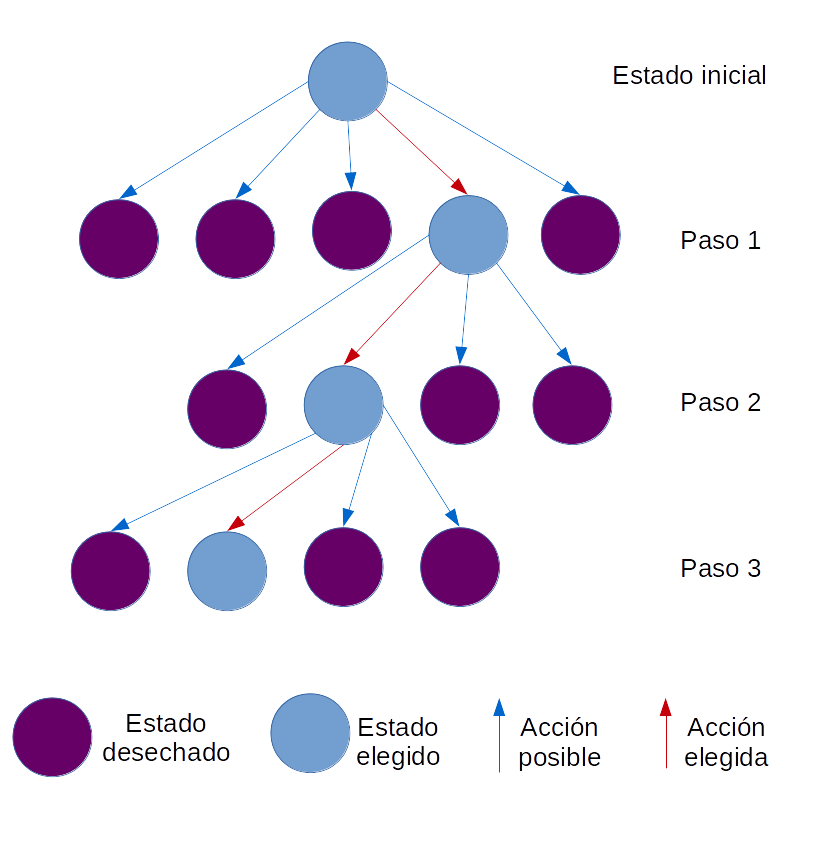
\includegraphics[scale=0.5]{img/arbol-busqueda}
\caption{Árbol de búsqueda para el método planteado
\label{fig:searchtree}}
\end{figure}

Esto es así porque un componente de backtracking podría encarecer el algoritmo en cuanto a tiempo de ejecución, además de que podemos decir que trabajamos en el sistema siempre con el mismo mapa de tiles para poder comprobar las colisiones entre los mapas.

Aún así, en cada paso del algoritmo se guarda el movimiento que se realiza. Con ésto, se ha implementado la forma de reconstruir un mapa a partir de una serie de movimientos consecutivos. Con esto, comentaremos en el capítulo de trabajo futuro, una forma factible de poder realizar backtracking.

Para la elaboración de este proyecto no se vió necesario, ya que los resultados que se obtienen con el sistema tal cual está, son bastante buenos y adecuados al enunciado, además de que añadiría un componente de complejidad extra.
